\label{ch:impl}
This chapter details the implementation of the AMBA-AHB at the ESL together with its proof that it is a sound abstraction of the RTL. As with the Wishbone bus, the protocol can not be directly implemented without the use of so called agents. They allow for flexibility by allowing any master/slave using a blocking port to be connected to the bus without explicitly having to implement the protocol themselves. The AMBA-AHB is a complicated protocol/architecture which would require extensive design effort and testing to implement from scratch. For this reason it was decided to use a trusted existing open source implementation of the interconnect, including arbiter and decoder \cite{ahbsys}. The existing architecture and the agents are described in section \ref{sec:hardover}. The biggest challenge in representing the AHB with SystemC-PPA is when multiple masters are introduced to the design. The masters are restricted by arbitration, but are otherwise free to act independently from eachother. This leads to a great deal of parallelism and an exponential increase in possible outputs/states for each added master, if the system is viewed as a whole. Just to paint the picture, consider the FSM in figure \ref{fig:rafsm}. The transition $Idle Phase\rightarrow Request Phase$ has 4 possibilities for two masters. However, if one master transitions then the possibility of transition $Idle Phase\rightarrow Request Phase$ for the other master must be accounted for in each clock cycle throughout the whole FSM. The full ESL description and what this challenge entails is covered in section \ref{sec:syslev}. The refinement of the formal properties generated for the design is described in section \ref{sub:refine}. System simulations at both levels are described in section \ref{sec:sim} with the generator introduced in section \ref{sec:generator}.

\newpage
\section{Hardware overview}
\label{sec:hardover}
\begin{figure}[hbt]
    \begin{center}
        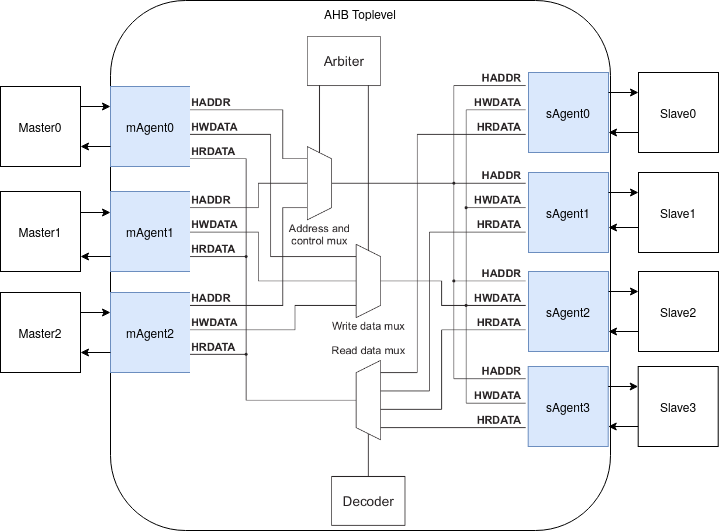
\includegraphics[width=0.8\textwidth]{figs/hw/Hw_toplevel.png}
    \end{center}
    \caption{Hardware toplevel with 3 masters and 3 slaves connected}
    \label{fig:hw_toplev}
\end{figure}

\subsection{Existing hardware}
\label{sub:exist}
The existing hardware is a stripped and slighlty modified version of the ahb system generator \cite{ahbsys}. Only the modules concerning the arbiter, decoder and interconnect are taken from this design. This architecture is a trusted implementation of the AHB protocol, and is often referred to when students inquire online about the AHB implementation. It is designed to be generated for a selected number of master and slaves so it is perfect for the purpose of this thesis. It provides the option to select between six modes of arbitration; Fixed, Round Robin and random. The remaining three are the modified versions of these. With the modified version a grant is not taken away when first given, if the request remains asserted. This implementation will be using Fixed modified, to simplify a possible implementation of burst transfers. The maximum number of masters and slaves on this arhcitecture is 15 each. This hardware is what connects the agents together in figure \ref{fig:hw_toplev} and can be referred to as the AHB- or bus matrix. A bottom up abstraction was done on this design, which lead to the discovery of an erroneous slave respone from the default slave. The design provided a constant error signal on \textbf{HRESP} regardless of encoding on \textbf{HTRANS[1:0]}. While it still provided the two cycle error response properly, it did not provide the zero cycle okay response as described in section \ref{subsec:slvresp}. This may go undetected in simulation if no master is explicitly dependent on the zero cycle okay response being correct. In this case it would greatly complicate verification, for this reason it was corrected.  
 
  
\subsection{Master agent}
The master agent receives a payload representing a subset of the AHB master interface from the master. Parts of this subset is defined with different types than the original interface to enhance readability and abstraction on the ESL. Table \ref{tab:mpayload} highlights these changes. 
\begin{table}[hbt] 
  \label{tab:mpayload}
  \begin{tabular}{|p{25mm}|r|p{10cm}|} 
  \hline
  \textbf{Signal} & \textbf{Type} & \textbf{Content} \\
    \hline
  \textbf{HADDR} & unsigned int & 32-bit \\
    \hline
  \textbf{HWDATA} & unsigned int & 32-bit \\
    \hline
  \textbf{HWRITE} & enum & AHB\_READ, AHB\_WRITE \\
    \hline  
\textbf{HSIZE} & enum & MT\_B (byte), MT\_H (halfword), MT\_W (word) \\
    \hline
  \end{tabular}
\caption{Master out payload}
\end{table}

The reason behind using a subset is that the remainder of the signals are either hardwired or provided by the agent. The response data payload consists of \textbf{HRDATA} and \textbf{HRESP}. \textbf{HRESP} is included in the payload at a cost of latency for consecutive writes from the same master. Instead of providing new address and data the agent needs to report success to the master. Reporting success back to the master is crucial since the master could possibly attempt to write to an unknown location. Repeated attemps or dependencies may lead to system crash or deadlock. 
\newline
\begin{wrapfigure}{l}{5.5cm}
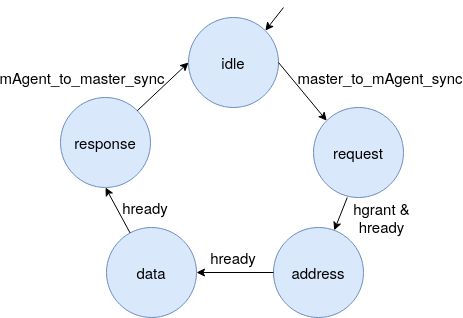
\includegraphics[width=5.5cm]{figs/hw/mAgent_FSM.png}
\caption{Master agent FSM}\label{fig:rafsm}
\end{wrapfigure}  

As seen from figure \ref{fig:rafsm} extra states are added to the system to enable the communication between the agent and the master. The agent will always be ready for a payload from the master, and when received it advances to the \textit{Request Phase}. At this point the agent has already translated and written the entire payload to the bus. In the \textit{Request Phase} \textbf{HBUSREQx} remains asserted until both \textbf{HGRANTx} and \textbf{HREADY} is set. When both signals are set the agent proceeds to the \textit{Address Phase} where it encodes \textit{nonsec} on its \textbf{HTRANS[1:0]} until \textbf{HREADY} is set. Otherwise \textbf{HTRANS[1:0]} will always be encoded with \textit{idle}. The agent proceeds to the \textit{Data Phase} where it waits until the \textbf{HREADY} is again set before sampling \textbf{HRDATA} and \textbf{HRESP}. It proceeds to the \textit{Response Phase} where it writes the payload to its master and returns to \textit{Idle Phase}. \\
\newline
The entire payload is written to the bus already in the Request Phase to enable a higher level of abstraction in the bus matrix. This way it is not necessary to keep track of which master is granted at all timepoints, greatly increasing abstraction. It can safely be done as described so long as the encoding of \textbf{HTRANS[1:0]} is used in a correct manner. The only overhead is that it reduces throughput, but this is already reduced as a consequence of the blocking port combined with the need to report status back to the master. In a system with bursts implemented, the encoding of \textbf{HTRANS[1:0]} will also include \textit{seq}, but this feature is explored in chapter (ref something). Because of the decision to report status back to master in every transfer, the response data is sampled regardless of the transfer direction. This reduces ESL and verification complexity significantly, at the cost of one extra clock cycle latency for reads. 

\subsection{Slave agent}
Similarily to the master agent, only a subset of the AHB slave interface is written from the slave agent to the slave. This is the same payload as master agents. 

\begin{wrapfigure}{l}{5.5cm}
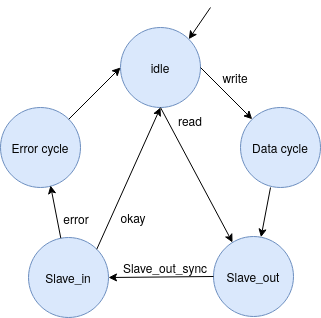
\includegraphics[width=5.5cm]{figs/hw/sAgent_FSM.png}
\caption{Master agent FSM}\label{fig:rsfsm}
\end{wrapfigure}  

As figure \ref{fig:rsfsm} shows the slave agent FSM is more complex than that of the master agent. To make the slave agent comply with the AHB protocol it needs to both obey the rules of the transfer phases and provide the proper response while communicating with its slave. A slave agent is always ready to receive a payload from its master, namely the AHB matrix. Starting from the \textit{idle\_phase} the agent stays idle until it is both selected and the encoding of \textit{nonseq} is detected on its inputs. When true it samples address and control signals from the AHB matrix and proceeds to the \textit{data cycle} where it samples the data. After sampling the data, the payload is written to the slave out port named \textit{sAgent\_to\_slave}. At this point the agent waits for a handshake, which should normally occur instantly but that is not a requirement. After the handshake is received it proceeds to wait for the response data and status from the slave, as with the output there is not a strict requirement on the wait time but it is recommended to keep the wait states under 16 cycles in total. The slave agent deasserts \textbf{HREADY} throughout its entire conceptual data phase, and zeroes \textbf{HRDATA} one clock cycle after asserting \textbf{HREADY}. \\
\newline
The slave agent may at any given timepoint be operated by another master. This is why the slave deasserts its \textbf{HREADY} throughout its entire conceptual data phase. It is standard for a slave to introduce wait states. As with a DRAM module, there are delays associated with activating a row (insert data). As with DRAM this delay is minimized in sequental address transfers using bursts. In contrast to the diagram in figure \ref{fig:transfer}, the conceptual data phase of the slave agent does not include the assertion of \textbf{HREADY}. This is a slight misnomer since the data phase does infact include the assertion as seen from the properties. It is however not included in the FSM to not diffuse the differences between the states. The \textit{idle\_phase} and \textit{error cycle} only differentiate in the value of \textbf{HRESP}. Although the assertion of \textbf{HREADY} technically is a part of the data phase, it is however beneficial to highlight that these are seperate states, as they are represented as such in the RTL description. The zeroing of \textbf{HRDATA} is a design choice to increase abstraction. 
\newpage

\section{System level representation}
\label{sec:syslev}
\begin{figure}[hbt]
    \begin{center}
        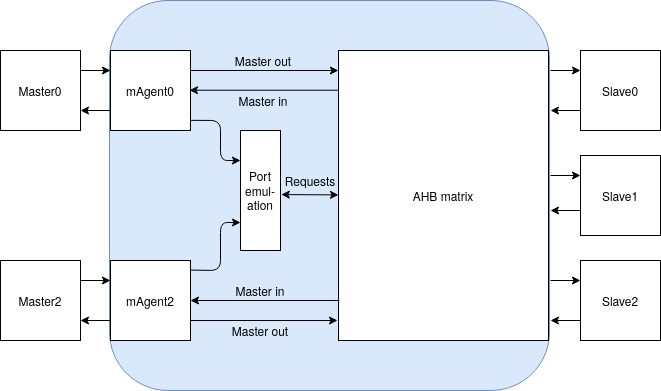
\includegraphics[width=0.8\textwidth]{figs/ESL/Syslev.png}
    \end{center}
    \caption{ESL toplevel with 2 masters and 3 slaves connected}
    \label{fig:esl_toplev}
\end{figure}

Describing the AHB system with SystemC-PPA in a single cluster is no longer feasible when more than one master is connected to the bus matrix. The master agents must be contained within their own clusters, or PPAs so that it does not need to be accounted for every possible combination. Since only one slave may be operated at a time, including them in the bus matrix PPA reduces the overhead. The interface between the master agent and the bus matrix have signals with mostly identical values for all masters, the exception is \textbf{HGRANTx}. This signal is purely combinational in the implementation, meaning that it changes its value within the same clock cycle as its initiator. Using any combination of existing ports there was not found any manner to represent this interface for multiple masters. The decision was made to create the properties bottom-up, to determine if the interface could be represented using existing ports and if not, where the gap is. Gap free verification was used for this purpose, with the style of generated properties in mind. 

\subsection{Bottom-up abstraction}
The first challenge of carrying out the GFV process is determining the CSM of the AHB. It has to be represented in such a way that it is feasible to describe at the ESL. Looking at other formal verification efforts made on the AHB \cite{ahbformal}, it can be seen that the real FSM of an AHB is incredibly complex. Furthermore, it is described how the state of the bus is dependent not just on state and inputs but on previous states as well. It is necessary to know the state of the bus, namely if there is a transfer being carried out or not. It is not as simple as paying attention to bus ownership since there is no way of knowing if there is a transfer in progress when the default master owns the data bus, without looking at past values on \textbf{HTRANS[1:0]}. One would furthermore need to constrain the design to establish how far into the past to look. One could go with the suggested maximum delay of slaves for 16 clock cycles. A much simpler solution is to define the master agents states as outputs to their clusters, and define this as inputs to the main cluster. By only concerning with which masters are requesting and where the data goes, the CSM can be made quite simple. If one was concerned with which master owned the address and which master owned the data bus at all times it would lead to state explosion, making an ESL description unfeasible even for a low number of masters.     

\begin{figure}[ht!]
	\centering
	\begin{minipage}[t]{0.49\textwidth}
		\centering
		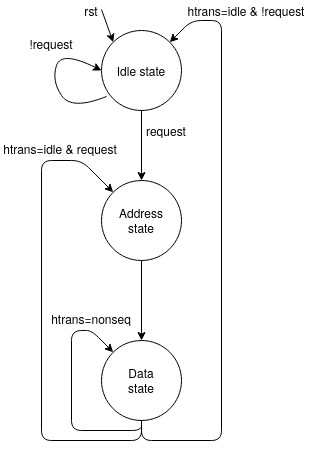
\includegraphics[scale=0.5]{figs/ESL/Bus_fsm_new.png}
		\captionof{figure}{Abstract CSM}
		\label{fig:OC}
	\end{minipage}
	\begin{minipage}[t]{0.49\textwidth}
		\centering
		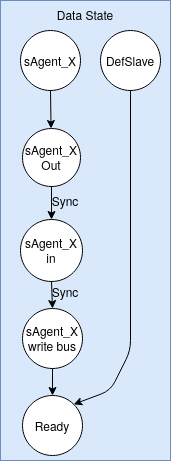
\includegraphics[scale=0.5]{figs/ESL/Data_state.png}
		\captionof{figure}{Detailed data state CSM}
		\label{fig:eslfsm}
	\end{minipage}
\end{figure}

By using a fixed priority arbitration scheme it is simple to determine which master is granted the bus. By dividing the transfer into three main states with the data state divided into five further, there is no need to impose any constraints on wait states. The bus is ready (\textbf{HREADY} is set) at the end of each state and any request is ignored unless the bus is ready. The states can be defined as follows:
\begin{itemize}
\item Idle state: No transfer in progress.
\item Address state: One master is in the address phase of the transfer, no masters are in the data phase. There is no trigger for the next state as the bus/slaves will always be ready here. 
\item Data state: One master is in the data phase of the transfer. This state is broken down into five substates per slave, with default slave as exception.  
\end{itemize}

It is worth noting that in the idle and address state the bus/slaves are always ready. The payload is transferred between the states using visible register which are named \textit{AS\_regs} for the address state and \textit{DS\_regs} for the data state. The Data state is divided into several important states to describe the transaction between the slave and its agent while simultaneously describing all necessary outputs. The default slave has only two states and they are self explanatory because of the two cycle error response. The remaining slave agents are explained by the following:
\begin{itemize}
 \item First state: There is one clock cycle delay required to allow the slave agent time to sample the possible data provided in the data phase.
 \item Second state: Slave agent writes payload to slave using blocking write. 
 \item Third state: Slave agent reads back from slave using blocking read.
 \item Fourth state: Slave writes payload back to bus. This requires two cycles due to the possibility of error, error cycle was removed from master agent due to inconsistencies in simulation. For this reason information on error is only contained within the visible registers handling response.   
 \item Fifth state: The bus is ready, payload is sampled, requests are handled and next state is determined based on the value of \textbf{HTRANS[1:0]}, which has been added to \textit{AS\_regs} alongside the payload. 
\end{itemize}

It is easy to see that the differentiation between read and write within the AHB matrix would lead to the double amount of data states, with the gain being one clock cycle saved in the case of a read. The entire design is represented by this CSM using only properties with length $t=1$ so determining the output is straightforward with the exception of \textbf{HGRANTx}. As this is an output that is not stored in a register its value updates in the same clock cycle as its instigator. This is not a problem to model in the properties themselves, but this representation does not allow for any sound abstraction between the RTL and ESL. Determining the value of \textbf{HGRANT} in the next clock cycle is not feasible in this implementation. One would have to account for every \textbf{HBUSREQx} as an assumption at $t+1$ in every property. An alternative could be to enable this output through a register but this would lead to unpredictable behaviour. This output is simply determined as the output of a function \textit{mx\_grant} and is at the ESL represented using an enum. \\
\newline
The design choice to zero \textbf{HRDATA} and modify the default slave response entails that \textbf{HRDATA} and \textbf{HRESP} will be zero unless it is in the fourth or fifth concepceptual data state. After adding all determination requirements and proving completeness the properties show that the interface between the master agents and AHB matrix cannot be represented using a single existing SystemC-PPA port. Referring back to section \ref{subsec:ports} there is a choice between three ports. For clarity the implications of using each port is commented.
\begin{itemize}
 \item \textit{Shared}: Explicit synchronization is needed to ensure that the value of \textbf{HREADY} and \textbf{HGRANTx} is neither overwritten nor obsolete. A solution was experimented with to highlight the increased abstraction. It was not successful without introducing illegal statemets with respect to SystemC-PPA, even when disregarding the combinational response of \textbf{HGRANTx}.   
 \item \textit{MasterSlave}: With MasterSlave some implicit synchronization is enabled. However, in this system one would be left with one of two choices. The bus matrix is the slave, or the master agents are the slaves. In either case the values of \textbf{HGRANTX} and \textbf{HREADY} would need to be representing correct values in every cycle. One side must always be ready for communication, so neither alternative is worth concidering.  
 \item \textit{Blocking}: The blocking port can be used to represent all signals functionally, but with blocking ports alone there are some issues. On the master agent side \textbf{HBUSREQx}, \textbf{HGRANTx} and \textbf{HREADY} can be represented both functionally and in the properties by the notify and wait used for synchronization. On the bus matrix side the functionality could be represented, but not the properties due to the states implied by each port. They all require their own state, and in turn a separate clock cycle to assert and deassert these signals.
\end{itemize}

The remaining option is to emulate a single compound port using a combination of shared and blocking ports.

\subsubsection{Combinatory port emulation}
When examining the FSM in figure \ref{fig:rafsm} it is seen that the traversal of the master agent state machine is always blocked by an input signal. The \textit{Request-}, \textit{Address-} and \textit{Data\_phase} are blocked by the AHB matrix's response signals \textbf{HREADY} and \textbf{HGRANTx}. Although the value of \textbf{HGRANTx} is impossible to determine effectively in the next clock cycle, its functionality with respect to the state machine can still be properly represented using a blocking port. The handshake from the master agents side represent the request, whereas the handshake from the AHB matrix side represent \textbf{HGRANTx} and \textbf{HREADY}. Due to the pipeline nature of the bus, a request can occur at any main state of the bus as seen from figure \ref{fig:OC}. This creates the requirement of a separate output representing \textbf{HREADY} alone, to allow for state machine traversal after bus has been granted. Only one port read can be represented in each clock cycle for blocking ports. Due to each master agent requiring their own port for each of the cases, it is necessary to contain these ports in a seperate module, and treat it as a new type of port interface.
This port determines internally which master agent gets granted/unblocked with a simple fixed priority arbitration scheme. The final issue is having the port correctly represent updated requests. For this reason the port waits for a synchronization signal (handshake) from the AHB matrix. When this handshake is received the port peeks on all its request inputs and forwards this information to the AHB matrix through a \textit{Shared} interface, while simultaneously unblocking the highest priority requesting agent and every \textbf{HREADY} port waiting for a synchronization signal. Special care has been taken to ensure that this happens in an atomic and synchronized manner.   
\begin{wrapfigure}{l}{5.5cm}
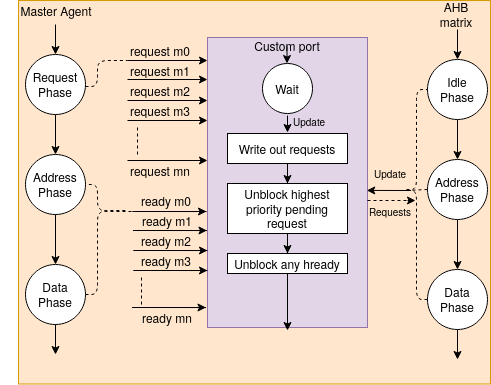
\includegraphics[width=5.5cm]{figs/ESL/port_diagram.png}
\caption{Illustration of port connection}\label{fig:cport}
\end{wrapfigure}

The port in figure \ref{fig:cport} is illustrated using the actual port directions in the ESL description, raher than the direction they symbolize. The inputs representing \textbf{HREADY} must be atomically unblocked which only happens when there is a pending handshake. To check for this the \textit{peek} function must be called, which is only available for reader ports. On the AHB matrix side the synchronization call to update the requests must always hand over control to the port by use of a wait function, which is only unconditionally called by use of a write port. When control is handed back to the AHB matrix the updated requests can be fetched from a shared port. 

\subsubsection{Master agent}
\begin{wrapfigure}{l}{5.5cm}
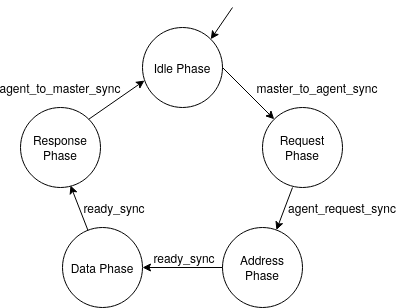
\includegraphics[width=5.5cm]{figs/ESL/mAgent_ESL.png}
\caption{master agent FSM}\label{fig:eafsm}
\end{wrapfigure}
The master agent is at the ESL in a quite simple manner using blocking ports to determine important states. All states from figure \ref{fig:rafsm} are deemed important states. They are all needed to communicate with the individual states of the bus matrix, or their masters. Transitions between the states are dependant on the synchronization signals alone, and all remaining interface signals are passed through shared ports. The generated properties are refined with minimal effort and proven to be a sound abstraction of the master agent RTL.  \\
\newline  

\subsubsection{Bus matrix}
The bus matrix has three main states as seen from figure \ref{fig:OC}. There is only one single communication with the emulated port in each of the three states. 
\begin{lstlisting}
   update_requests->try_write(true, sync, "idle_state");
   requests_in->get(reqs);
\end{lstlisting}

The non-blocking write 


The bus matrix is a more complex implementation, as can be seen from figure \ref{fig:eslfsm}.

 All shared outputs are written, or determined in all of the states to enable the generated properties to satisfy the completeness criterion. The remaining signals to the interface are implicitly determined at all times by the blocking port. To aid in understanding section \ref{sub:refine} an overview of important signals is provided. 

\begin{table}[hbt] 
  \begin{tabular}{|p{3cm}|r|p{7cm}|} 
 \label{tab:impsig}
  \hline
  \textbf{Signal} & \textbf{Type} & \textbf{Description} \\
    \hline
  \textit{update\_requests} & blocking\_out & Uses non blocking write to signal the emulated port to update requests. \\
    \hline
  \textit{requests\_in} & shared\_in & A compound of all pending requests provided by the emulated port \\
    \hline
  \textit{AS\_regs} & visible reg & The payload from the master but including \textbf{HTRANS[1:0]}. Stores the values of granted agent in its address phase. \\
    \hline  
\textit{DS\_regs} & Visible reg & The payload from the master, stored for any master in its data phase.  \\
    \hline
\textit{resp} & Visible reg & stores response from the slave. \\
    \hline
  \end{tabular}
\caption{Important signals}
\end{table}
  

\subsection{Refining properties}
\label{sub:refine}



\section{Simulation}
\label{sec:sim}

\subsection{Starvation}

\section{Generator}
\label{sec:generator}
